\section{Task 1}

This is not just copy pasted image. (still do not know why did I do this)

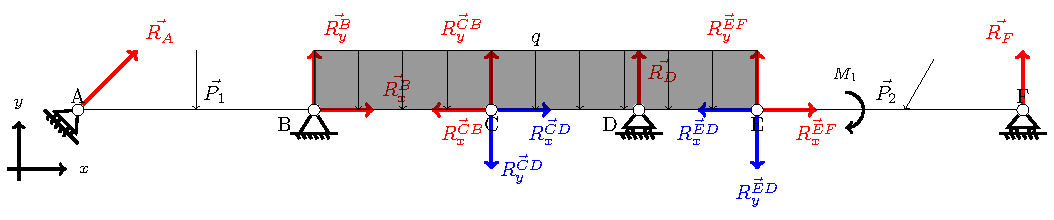
\includegraphics[width=\linewidth]{graphics/task1.pdf}

\subsection*{Research object:}
\begin{enumerate}
    \item 3 rigid bodies: $AC$, $CE$, $EF$.
    \item $A$, $D$, $F$ are roller supports
    \item $B$ is a hinge support
    \item $C$ and $E$ are pin connections
\end{enumerate}

\subsection*{Method: }

Statics, the whole stud is in equilibrium.

\subsection*{Force analysis:}

\begin{enumerate}
    \item $A$ --- $R^{A}_x = R^{A}_y = R^{A} \cdot \frac{\sqrt{2}}{2}$
    \item $B$ --- $R^{B}_x, R^{B}_y$
    \item $C$ --- $|R^{CB}_x| = |R^{CD}_y| = |R^{C}_y|$, $|R^{CD}_x| = |R^{CB}_x| = |R^{C}_x|$
    \item $D$ --- $R^{D}_y$
    \item $E$ --- $|R^{ED}_x| = |R^{EF}_x| = |R^{E}_x|$, $|R^{ED}_y| = |R^{ED}_y| = |R^{E}_y|$
    \item $F$ --- $R^{F}_y$
    \item $P_1$ --- $P_{1x} = 0$, $P_{1y} = - P_1$
    \item $F_q$ = $q \cdot BE$
    \item $M_1$
    \item $P_2$ --- $P_{2x} = - P_2 \cdot \cos (\pi / 4)$, $P_{2y} = - P_2 \cdot \sin (\pi / 4)$
\end{enumerate}

\subsection*{Unknowns:}
\begin{enumerate}
    \item $R^{A}$, $R^{B}_y$, $R^{C}_x$, $R^{C}_y$, $R^{D}_y$, $R^{E}_x$, $R^{E}_y$ $R^{F}_y$
\end{enumerate}

\subsection*{Solution:}

\begin{enumerate}
    \item Body $AC$
          Equations by axis and moment around $A$:
          \begin{align}
              \begin{cases}
                  R^{A} \cos (\pi / 4)  +R^{B}_x - R^{C}_x                              = 0 \\
                  R^{A} \sin (\pi / 4) - P_1 + R^{B}_y + R^{C}_y - q \cdot BC = 0           \\
                  - P_1 \frac{AB}{2} + R^{B}_y \cdot AB + R^{C}_y \cdot AC - q \cdot BC \cdot \frac{BC}{2} = 0
              \end{cases}
          \end{align}
    \item Body $CE$
          Equations by axis and moment around $C$:
          \begin{align}
              \begin{cases}
                  R^{C}_x - R^{E}_x = 0                       \\
                  -R^{C}_x + R^{E}_y - q \cdot CE + R^{D} = 0 \\
                  R^{E}_y \cdot CE - q \cdot CE \cdot \frac{CE}{2} + R^{D} \cdot CD = 0
              \end{cases}
          \end{align}
    \item Body $EF$
          Equation by axis and moment around $E$:
          \begin{align}
              \begin{cases}
                  R^{E}_x - P_2 \cos(\pi/3) = 0          \\
                  -R^{E}_y - P_2 \sin(\pi/3) + R^{F} = 0 \\
                  - M_1 - 2.5 P_2 \sin(\pi/3) + R^{F}_y \cdot EF = 0
              \end{cases}
          \end{align}

    \item Solved these systems using python

\end{enumerate}

\subsection*{Answer:}

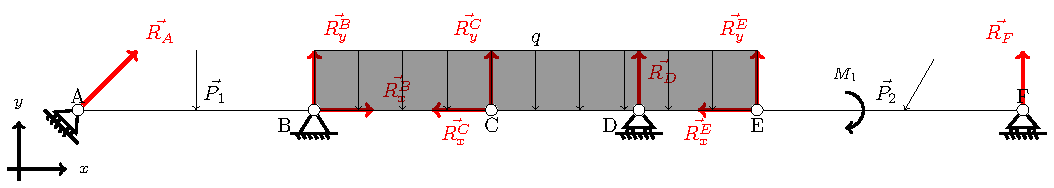
\includegraphics[width=\linewidth]{graphics/task1final.pdf}

\begin{answer}
    \begin{align*}
        R^{A} = 4.680229388568428     \\
        R^{B}_x = 5.690578061834697   \\
        R^{B}_y = 14.378015477614287  \\
        R^{C}_x = 9.000000000000002   \\
        R^{C}_y = -1.4874374157795929 \\
        R^{D} = 3.7407658144959157    \\
        R^{F} = 16.660254037844386    \\
        R^{E}_x = 9.000000000000002   \\
        R^{E}_y = 1.0717967697244912
    \end{align*}

\end{answer}

